\BigLetter{A}{ progressively} increasing challenge in high performance computing (HPC) is how to store the large amount of data on disk efficiently, especially with the ubiquitous enthusiasm for Big Data Analysis (BDA) frameworks, within the area of influence. A commonly used distributed computation framework for BDA is Apache's Hadoop\cite{PageHadoop}, where data access is based on the Hadoop Distributed File System (HDFS) \cite{Shvachko:2010:HDF:1913798.1914427} and the primary execution model is based on MapReduce\cite{Dean:2008:MSD:1327452.1327492}. These frameworks are developed under different circumstances, and with different purposes compared to what they are presently used.
\newline

HDFS, as well as the Google File System \cite{Ghemawat:2003:GFS:945445.945450}, follows a centralized architectural master/slave organization (described in \cite{Tanenbaum:2006:DSP:1202502} and briefly in \cite{Wilkinson:1998:PPT:289352}) where what is denoted as NameNode acts as the master. This server maintains attributes such as permissions and namespace tree for slaves. Also, it implements a proxy to handle operations realised on the file system at the slaves. 
\newline

Writing to the Hadoop file system can likely cause what's known as the data residual problem (Figure \ref{fig:data-residual}). Thus, semantically correlated or coherent data can be distributed across different servers. Hadoop is implemented using a conventional file system approach, \ie fixed sized blocks of 64MB. 
\newpage

\begin{figure}
	\centering
	\hspace*{15mm}
	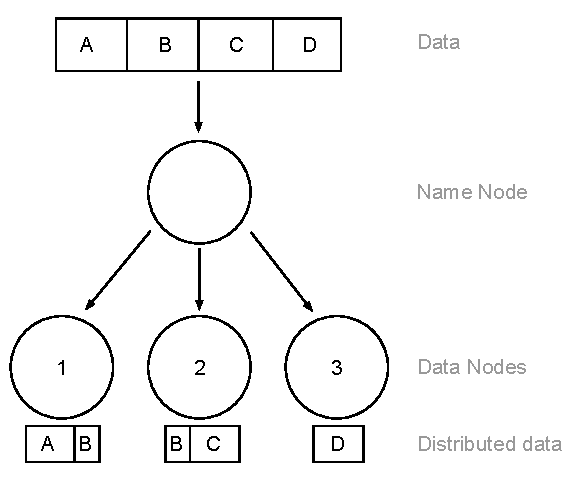
\includegraphics[scale=0.8]{pdf/data-residual.pdf}
	\caption[HDFS data residual problem]{HDFS data residual problem which ultimately requires Data Node 1 and 2 to exchange data for a consistent processing of block B, leading to an increased I/O cost. \label{fig:data-residual}}
\end{figure}

As a matter of fact, the only case where data partitioning is ensured to be avoided is when \textit{the size of the data} modulo \textit{the block size} is equal to zero. As a consequence, individual computer scientist are required to implement a network communication protocol between the slaves to handle this problem, which typically causes increased latency. The goal is to ensure a consistent view and process of the coherent data representations.

\section{Problem definition} \label{sec:problem}
\begin{quotation}
\hspace*{-7mm}
\textit{Firstly, analyze and investigate whether a distributed parallel file system that efficiently hides latency and reduce IO-cost is feasible. Secondly, if such a system is feasible implement a prototype in a sensibly selected language, architecture and environment.} \newline
\end{quotation}

\section{Related work} \label{sec:related}
Existing implementations and research projects within the field of big data analysis frameworks and distributed parallel file systems relevant to this project will be described in this section, including the once previously mentioned.

\subsection*{Hadoop}
Hadoop was originally described in 2010 by Shvachko \etal \cite{Shvachko:2010:HDF:1913798.1914427}. The Apache and Yahoo! developed framework is designed to store and analyze enormous datasets. It provides the distributed hierarchical file system with directories and archives HDFS, as data access layer (DAL) and a primary execution model based on the programming paradigm MapReduce (sharing this feature with the following computing platform), outlined in Definition \ref{def:mapreduce}.
\vspace*{2mm}

\begin{definition}[MapReduce] \label{def:mapreduce}
\textit{A programming paradigm and an associated implementation presented by Dean and Ghemawat} \cite{Dean:2008:MSD:1327452.1327492} \textit{used for data generation, analysis and processing. Fundamentally it is assembled by two separate user specified functions:} \texttt{map} \textit{and} \texttt{reduce}\textit{, which at execution time are parallelized automatically.}
\end{definition}
\vspace*{2mm}

HDFS implements a master/slave architecture where the NameNode server acts as the master and the DataNodes are the slaves. Metadata and application data are stored separately on respectively master and slave. Having a stateful master without replication is a single point of failure  as described by Yahoo! in the Hadoop developer tutorial:

\begin{quotation}
	\textit{"The single point of failure in a Hadoop cluster is the NameNode $\ldots$ loss results in cluster unavailability. The permanent loss of NameNode data would render the cluster's HDFS inoperable."}\cite{YahooDocumentation}
\end{quotation}

Additionally it's a potential bottleneck in a system, but in this project it's a tradeoff between throughput and accessibility.

\subsection*{Facebook (Hadoop)}
Approximately 40\% percentage of all incidents at the Facebook Data Warehouse is somewhat Hadoop related (Figure \ref{fig:fb-hadoop-incidents}), many of those is due to the single point of failure (SPOF) error at the NameNode, which causes more or less the whole Hadoop cluster to be unavailable and thus not correctly functioning. Improving HDFS and SPOF error at the NameNode is therefor an essential task to ensure that the ecosystem are efficient and reliable.

\begin{figure}[h!]
	\centering
	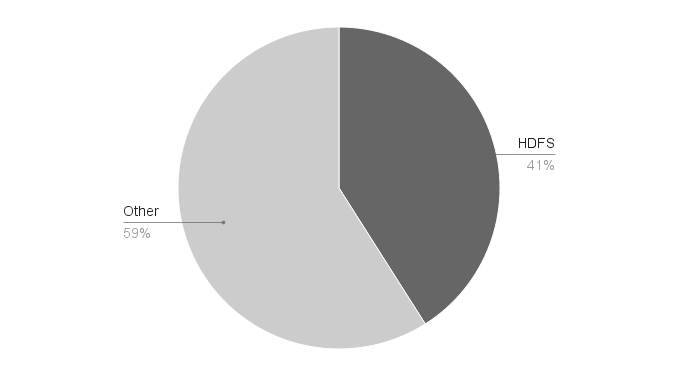
\includegraphics[scale=0.48]{img/fb-hadoop-incidents.png}
	\caption[Incidents at Facebooks Data Warehouse]{Incidents at Facebooks Data Warehouse by percentage at the responsible part, others including user specified jobs etc.\cite{FacebookHadoopImprovement}. \label{fig:fb-hadoop-incidents}}
\end{figure}

\newpage
Facebooks engineers designed a solution based on a so-called Avatar\-node, as a functioning hot fail-over solution, turning the existing NameNode into a highly-available server. The open source Avatarnode is essentially two NameNodes wrapped in an Apache ZooKeeper\footnote{Apache ZooKeeper\cite{PageZookeper} is a centralized service provider for configuration information and naming etc.} instance, with support for manual failover. The two NameNode instances behave as an active one and a standby with internal virtual IP address (VIP), handled by ZooKeeper, \ie each client request is initialized through that to get the VIP of the primary node (Figure \ref{fig:facebook-avatarnode}).
\newline

Synchronization between the active and the standby NameNode instance is managed by a NFS (Network File Server).
\vspace*{3mm}

\begin{figure}[h!]
	\centering
	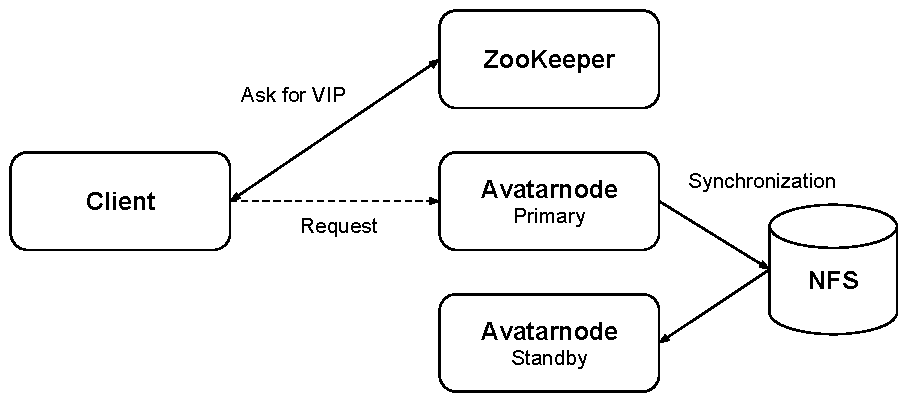
\includegraphics[scale=0.8]{pdf/facebook-avatarnode.pdf}
	\caption[Avatarnode: Facebooks Hadoop implementation]{Control flow of the AvatarNode and ZooKeeper with virtual IP address and network file server for synchronization. \label{fig:facebook-avatarnode}}
	\vspace*{3mm}
\end{figure}

Facebook claims that the solution leads to a projected result of 50\% lesser planned downtime, \ie a critical time where that part of the warehouse is unavailable. Though, one could certainly come up with new issues arising in this solution:
\begin{itemize}
	\item SPOF error reliability of the Apache ZooKeeper instance, since that is the only access-point now.
	\item SPOF error reliability of the NFS.
\end{itemize}

\subsection*{Hadoop 2.x}
Apache later released in Hadoop \textbf{2.x} \cite{Hadoop2xDocumentation} their solution to the single point of failure problem which they have described as: 

\begin{quotation}
	\textit{"$\ldots$ if that machine or process became unavailable, the cluster as a whole would be unavailable until the NameNode was either restarted or brought up on a separate machine"}. 
\end{quotation}

The solution is based on redundant duplication of the NameNode, such that one machine acts as the active one serving clients and another as the full redundant standby, which allows a fast fail-over in the case that the Active one crashes. The synchronization of logs and state between the two masters can be accomplished in two different ways:
\vspace*{3mm}

\begin{enumerate}
	\item Having at least 3 or more relatively lightweight Quorum Journal Manager (QJM) daemons to tolerate the failure of a single machine, because each modification has to be written to a quorum based majority of the daemons
	
	Major problems in this solution are:
\begin{itemize}
	\item Synchronization (the communication or latency cost of it).
	\item Considerable increase in hardware\footnote{One new machine for the standby and presumably three for the QJMs.}.
\end{itemize}
	\vspace*{3mm}
	
	\item Another option is to use a shared network file server (NFS) storage (Figure \ref{fig:hadoop-2x-nfs}).
	\begin{figure}[h!]
		\centering
		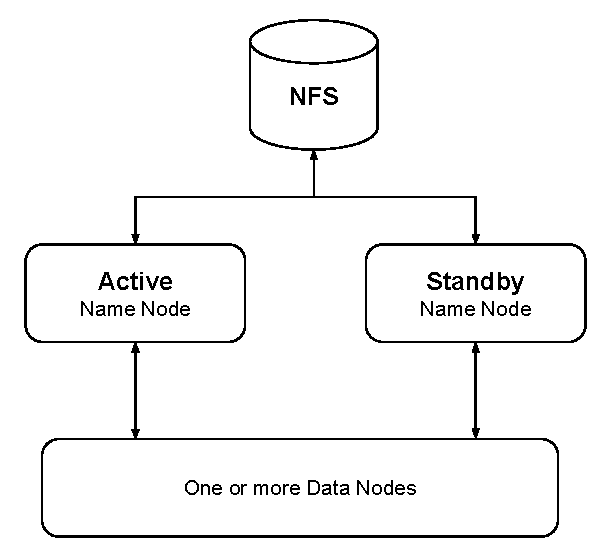
\includegraphics[scale=0.6]{pdf/hadoop-2x-nfs.pdf}
		\caption[Hadoop 2.x NFS solution]{Component diagram of the Hadoop 2.x NFS solution. \label{fig:hadoop-2x-nfs}}
	\end{figure}	

	This approach will undeniably mask the single point of failure (SPOF) error on the NameNode master by the cost and reliability to handle SPOF errors on the network file system abstraction, which in fact in most cases is a single server.
\end{enumerate}

\subsection*{Disco}
Mundkur \etal at Nokia Research Center published in 2011 a paper on their implementation of the distributed computing platform Disco\cite{PageDisco}\cite{Mundkur:2011:DCP:2034654.2034670}. Disco is an easy customizable MapReduce (Defintion \ref{def:mapreduce}) framework with regards to environment and requirements, designed for clusters of commodity server machines. Disco is likewise based on the master/slave architecture and relies on a standard file system and thus, deprioritizes persistent fault tolerance, achievable by a dedicated custom implementation. 
\newline

The single master pattern is as mentioned a single point of failure but is preferred due to consistency over availability (CAP theorem is outlined in \ref{def:cap}).
\vspace*{2mm}

\begin{definition}[CAP Theorem] \label{def:cap}
\textit{Eric Brewer presented in his keynote speech}\cite{Brewer2000} \textit{the CAP (Consistency, Availability, and Partition Tolerance) theorem that states, a distributed system (set of independent computers working together) only at any point in time can guarantee two of the three listed acronym properties, as illustrated in Figure \ref{fig:cap}.}

\begin{figure}[h!]
	\centering
	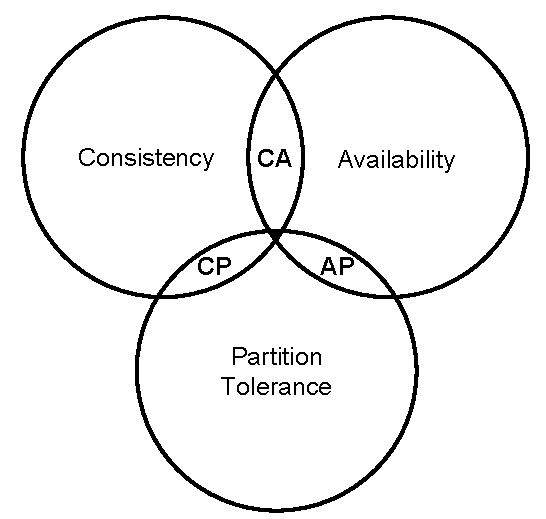
\includegraphics[scale=0.7]{pdf/cap.pdf}
	\caption{Illustrating the concept and limitations of CAP. \label{fig:cap}}
\end{figure}	
\end{definition}

\subsection*{Dynamo}
Dynamo is a highly available key-value storage system presented by Amazon engineers \cite{DeCandia:2007:DAH:1294261.1294281}. The system is implemented using an eventual consistency protocol and thereby sacrifices it under certain scenarios, by cause of availability. 

The reason for this choice is the \textit{"always-on"} user experience on core services on the Amazon platform that Dynamo is used to function. Dynamo uses consistent hashing (Definition \ref{def:ch}) to partition the key space across all available machines. A uniform distribution ultimately leads to a uniform load, assuming the key space access is not too skewed.
\vspace*{3mm}

\begin{definition}[Consitent hashing] \label{def:ch}
\textit{Engineer at Apache, White, describes in his blog post} \cite{PageWhiteCH} \textit{the purpose and demand for consistent hashing. It arose from the problems and limitations experienced with a naive hash-based key space distribution in a distributed system, where adding and removing machines in the network can be a catastrophe from a network bandwidth point of view, due to redistribution of the key space. In consistent hashing, only a fair share proportion from each of the machines is reassigned, while adding or removing machines.}
\end{definition}

\subsection*{Google File System}
Ghemawat \etal at Google describes the scalable distributed file system (GFS: Google File System) designed at implemented for primary developed for internal usage \cite{Ghemawat:2003:GFS:945445.945450}. 

The file system is designed to run on inexpensive commodity hardware like Dynamo and to provide fault tolerance. The architecture is a single stateful master and slave(s) organization, where the (GFS) master maintains all metadata file in the system. 
\newline

A vastly simplified design and sophisticated placement of data on the slaves, together with a strong recovery protocol has been prioritized compared to the risk of a single master (as previously explained). Communication between clients and the master are also widely reduced, by caching slave metadata for further intercommunication on the client eliminating the bottleneck effect on the master.
\vspace*{3mm}

\begin{definition}[Bottleneck effect] \label{def:bottle}
\textit{A part of a system is defined as a bottleneck if it critically limits the remaining system. This component usually has the lowest throughput of all.}
\end{definition}

\section{Proposal} \label{sec:proposal}
The knowledge, features, and compromises in the papers discussed and described in Related work provides the foundation for the research in the project. The ambition of the research is to first of all design a prototype of an alternative to the existing file archives used in big data analysis and secondly if possible to implement it.
\newline

The design of the architectural organization of the prototype is intended to eliminate the complications and issues in the existing solutions that has been described. A desired outcome is a substitute system eliminating data residuals with reduced I/O-cost and complexity and increased performance.
\newline

This can be achieved by splitting data semantically coherent at key positions by the file system, thus, data will be divided into arbitrarily sized chunks instead of fixed. Main challenges includes:
\vspace*{2mm}
\begin{itemize}
	\item Describing a domain specific model to characterize the data semantics.
	\item Defining a direct data mapping for storing and retrieval.
	\item Designing a system that scales as the data and request rate grows, \ie provides consistent and intelligent load balancing.
\end{itemize}

A feasible solution to reduce I/O-cost includes the mechanism of data cleaning, which is an important preprocessing step in big data analysis where \ie following actions can be performed:
\begin{itemize}
	\item Reformatting multidimensional scientific dataset such that identical features are grouped.
	\item Reducing noise.
	\item Transformation and dimensionality reduction (remove redundancy).
\end{itemize}
\vspace*{5mm}

The system seeks to perform the actions as mentioned above in real time since they are computationally simple on modern high-end processors and are attractive to perform before writing data to disk. 
\newline

Furthermore, a straightforward extension is to measure and store elemental statistics per dataset in a fashionable and state-of-the-art way. It is ultimately an ambition to integrate the same execution model as in \eg Hadoop and Disco, namely MapReduce around the implemented file archive to compose a full big data analysis framework alternative.

\section{Assumptions} \label{sec:assumption}
Following assumptions are constructed first and foremost to limit the prototype to the field of study relevant for this project and secondly to match the surrounding environment and settings.

\begin{itemize}
	\item The solution is targeted research and scientific datasets. 
	\item The solution is targeted and used for big data analysis.
	\item A full dataset is accessed, processed or modified at once.
	\item Individual data entries can be processed and analyzed independently and the order of data entries is irrelevant.
	\item The majority of the datasets are passive, \eg not quite accessed as much as expected in systems like GFS.
\end{itemize}

\section{Outline}
Part \ref{prt:sofa} explains the needs and requirements of the file archive for big data analysis based on the knowledge learned from analysis existing solutions in Chapter \ref{sec:introduction}. Additionally, it describes the architecture and design along with the implementation of the prototype. Part \ref{prt:extensions} explains the implementation of an extension build on top of the file archive based on the API described in Chapter \ref{chp:api}. Part \ref{prt:evaluation} finally, validates the correctness and measures the efficiency of the final solutions in addition to describing the plans for the future.